\chapter{The Journey}

Monte Cristo uttered a joyful exclamation on seeing the young men
together. “Ah, ha!” said he, “I hope all is over, explained and
settled.”

“Yes,” said Beauchamp; “the absurd reports have died away, and should
they be renewed, I would be the first to oppose them; so let us speak
no more of it.”

“Albert will tell you,” replied the count “that I gave him the same
advice. Look,” added he. “I am finishing the most execrable morning’s
work.”

“What is it?” said Albert; “arranging your papers, apparently.”

“My papers, thank God, no,—my papers are all in capital order, because
I have none; but M. Cavalcanti’s.”

“M. Cavalcanti’s?” asked Beauchamp.

“Yes; do you not know that this is a young man whom the count is
introducing?” said Morcerf.

“Let us not misunderstand each other,” replied Monte Cristo; “I
introduce no one, and certainly not M. Cavalcanti.”

“And who,” said Albert with a forced smile, “is to marry Mademoiselle
Danglars instead of me, which grieves me cruelly.”

“What? Cavalcanti is going to marry Mademoiselle Danglars?” asked
Beauchamp.

“Certainly! do you come from the end of the world?” said Monte Cristo;
“you, a journalist, the husband of renown? It is the talk of all
Paris.”

“And you, count, have made this match?” asked Beauchamp.

“I? Silence, purveyor of gossip, do not spread that report. I make a
match? No, you do not know me; I have done all in my power to oppose
it.”

“Ah, I understand,” said Beauchamp, “on our friend Albert’s account.”

“On my account?” said the young man; “oh, no, indeed, the count will do
me the justice to assert that I have, on the contrary, always entreated
him to break off my engagement, and happily it is ended. The count
pretends I have not him to thank;—so be it—I will erect an altar \textit{Deo
ignoto}.”

“Listen,” said Monte Cristo; “I have had little to do with it, for I am
at variance both with the father-in-law and the young man; there is
only Mademoiselle Eugénie, who appears but little charmed with the
thoughts of matrimony, and who, seeing how little I was disposed to
persuade her to renounce her dear liberty, retains any affection for
me.”

“And do you say this wedding is at hand?”

“Oh, yes, in spite of all I could say. I do not know the young man; he
is said to be of good family and rich, but I never trust to vague
assertions. I have warned M. Danglars of it till I am tired, but he is
fascinated with his Luccanese. I have even informed him of a
circumstance I consider very serious; the young man was either charmed
by his nurse, stolen by gypsies, or lost by his tutor, I scarcely know
which. But I do know his father lost sight of him for more than ten
years; what he did during these ten years, God only knows. Well, all
that was useless. They have commissioned me to write to the major to
demand papers, and here they are. I send them, but like Pilate—washing
my hands.”

“And what does Mademoiselle d’Armilly say to you for robbing her of her
pupil?”

“Oh, well, I don’t know; but I understand that she is going to Italy.
Madame Danglars asked me for letters of recommendation for the
\textit{impresari}; I gave her a few lines for the director of the Valle
Theatre, who is under some obligation to me. But what is the matter,
Albert? you look dull; are you, after all, unconsciously in love with
Mademoiselle Eugénie?”

“I am not aware of it,” said Albert, smiling sorrowfully. Beauchamp
turned to look at some paintings.

“But,” continued Monte Cristo, “you are not in your usual spirits?”

“I have a dreadful headache,” said Albert.

“Well, my dear viscount,” said Monte Cristo, “I have an infallible
remedy to propose to you.”

“What is that?” asked the young man.

“A change.”

“Indeed?” said Albert.

“Yes; and as I am just now excessively annoyed, I shall go from home.
Shall we go together?”

“You annoyed, count?” said Beauchamp; “and by what?”

“Ah, you think very lightly of it; I should like to see you with a
brief preparing in your house.”

“What brief?”

“The one M. de Villefort is preparing against my amiable assassin—some
brigand escaped from the gallows apparently.”

“True,” said Beauchamp; “I saw it in the paper. Who is this
Caderousse?”

“Some Provençal, it appears. M. de Villefort heard of him at
Marseilles, and M. Danglars recollects having seen him. Consequently,
the procureur is very active in the affair, and the prefect of police
very much interested; and, thanks to that interest, for which I am very
grateful, they send me all the robbers of Paris and the neighborhood,
under pretence of their being Caderousse’s murderers, so that in three
months, if this continues, every robber and assassin in France will
have the plan of my house at his fingers’ ends. I am resolved to desert
them and go to some remote corner of the earth, and shall be happy if
you will accompany me, viscount.”

“Willingly.”

“Then it is settled?”

“Yes, but where?”

“I have told you, where the air is pure, where every sound soothes,
where one is sure to be humbled, however proud may be his nature. I
love that humiliation, I, who am master of the universe, as was
Augustus.”

“But where are you really going?”

“To sea, viscount; you know I am a sailor. I was rocked when an infant
in the arms of old Ocean, and on the bosom of the beautiful Amphitrite;
I have sported with the green mantle of the one and the azure robe of
the other; I love the sea as a mistress, and pine if I do not often see
her.”

“Let us go, count.”

“To sea?”

“Yes.”

“You accept my proposal?”

“I do.”

“Well, viscount, there will be in my courtyard this evening a good
travelling britzka, with four post-horses, in which one may rest as in
a bed. M. Beauchamp, it holds four very well, will you accompany us?”

“Thank you, I have just returned from sea.”

“What? you have been to sea?”

“Yes; I have just made a little excursion to the Borromean Islands\footnote[18]{Lake Maggiore.}.”

“What of that? come with us,” said Albert.

“No, dear Morcerf; you know I only refuse when the thing is impossible.
Besides, it is important,” added he in a low tone, “that I should
remain in Paris just now to watch the paper.”

“Ah, you are a good and an excellent friend,” said Albert; “yes, you
are right; watch, watch, Beauchamp, and try to discover the enemy who
made this disclosure.”

Albert and Beauchamp parted, the last pressure of their hands
expressing what their tongues could not before a stranger.

“Beauchamp is a worthy fellow,” said Monte Cristo, when the journalist
was gone; “is he not, Albert?”

“Yes, and a sincere friend; I love him devotedly. But now we are
alone,—although it is immaterial to me,—where are we going?”

“Into Normandy, if you like.”

“Delightful; shall we be quite retired? have no society, no neighbors?”

“Our companions will be riding-horses, dogs to hunt with, and a
fishing-boat.”

“Exactly what I wish for; I will apprise my mother of my intention, and
return to you.”

“But shall you be allowed to go into Normandy?”

“I may go where I please.”

“Yes, I am aware you may go alone, since I once met you in Italy—but to
accompany the mysterious Monte Cristo?”

“You forget, count, that I have often told you of the deep interest my
mother takes in you.”

“‘Woman is fickle.’ said Francis I.; ‘woman is like a wave of the sea,’
said Shakespeare; both the great king and the great poet ought to have
known woman’s nature well.”

“Woman’s, yes; my mother is not woman, but \textit{a} woman.”

“As I am only a humble foreigner, you must pardon me if I do not
understand all the subtle refinements of your language.”

“What I mean to say is, that my mother is not quick to give her
confidence, but when she does she never changes.”

“Ah, yes, indeed,” said Monte Cristo with a sigh; “and do you think she
is in the least interested in me?”

“I repeat it, you must really be a very strange and superior man, for
my mother is so absorbed by the interest you have excited, that when I
am with her she speaks of no one else.”

“And does she try to make you dislike me?”

“On the contrary, she often says, ‘Morcerf, I believe the count has a
noble nature; try to gain his esteem.’”

“Indeed?” said Monte Cristo, sighing.

“You see, then,” said Albert, “that instead of opposing, she will
encourage me.”

“Adieu, then, until five o’clock; be punctual, and we shall arrive at
twelve or one.”

“At Tréport?”

“Yes; or in the neighborhood.”

“But can we travel forty-eight leagues in eight hours?”

“Easily,” said Monte Cristo.

“You are certainly a prodigy; you will soon not only surpass the
railway, which would not be very difficult in France, but even the
telegraph.”

“But, viscount, since we cannot perform the journey in less than seven
or eight hours, do not keep me waiting.”

“Do not fear, I have little to prepare.”

Monte Cristo smiled as he nodded to Albert, then remained a moment
absorbed in deep meditation. But passing his hand across his forehead
as if to dispel his reverie, he rang the bell twice and Bertuccio
entered.

“Bertuccio,” said he, “I intend going this evening to Normandy, instead
of tomorrow or the next day. You will have sufficient time before five
o’clock; despatch a messenger to apprise the grooms at the first
station. M. de Morcerf will accompany me.”

Bertuccio obeyed and despatched a courier to Pontoise to say the
travelling-carriage would arrive at six o’clock. From Pontoise another
express was sent to the next stage, and in six hours all the horses
stationed on the road were ready.

Before his departure, the count went to Haydée’s apartments, told her
his intention, and resigned everything to her care.

Albert was punctual. The journey soon became interesting from its
rapidity, of which Morcerf had formed no previous idea.

“Truly,” said Monte Cristo, “with your post-horses going at the rate of
two leagues an hour, and that absurd law that one traveller shall not
pass another without permission, so that an invalid or ill-tempered
traveller may detain those who are well and active, it is impossible to
move; I escape this annoyance by travelling with my own postilion and
horses; do I not, Ali?”

The count put his head out of the window and whistled, and the horses
appeared to fly. The carriage rolled with a thundering noise over the
pavement, and everyone turned to notice the dazzling meteor. Ali,
smiling, repeated the sound, grasped the reins with a firm hand, and
spurred his horses, whose beautiful manes floated in the breeze. This
child of the desert was in his element, and with his black face and
sparkling eyes appeared, in the cloud of dust he raised, like the
genius of the simoom and the god of the hurricane.

“I never knew till now the delight of speed,” said Morcerf, and the
last cloud disappeared from his brow; “but where the devil do you get
such horses? Are they made to order?”

“Precisely,” said the count; “six years since I bought a horse in
Hungary remarkable for its swiftness. The thirty-two that we shall use
tonight are its progeny; they are all entirely black, with the
exception of a star upon the forehead.”

“That is perfectly admirable; but what do you do, count, with all these
horses?”

“You see, I travel with them.”

“But you are not always travelling.”

“When I no longer require them, Bertuccio will sell them, and he
expects to realize thirty or forty thousand francs by the sale.”

“But no monarch in Europe will be wealthy enough to purchase them.”

“Then he will sell them to some Eastern vizier, who will empty his
coffers to purchase them, and refill them by applying the bastinado to
his subjects.”

“Count, may I suggest one idea to you?”

“Certainly.”

“It is that, next to you, Bertuccio must be the richest gentleman in
Europe.”

“You are mistaken, viscount; I believe he has not a franc in his
possession.”

“Then he must be a wonder. My dear count, if you tell me many more
marvellous things, I warn you I shall not believe them.”

“I countenance nothing that is marvellous, M. Albert. Tell me, why does
a steward rob his master?”

“Because, I suppose, it is his nature to do so, for the love of
robbing.”

“You are mistaken; it is because he has a wife and family, and
ambitious desires for himself and them. Also because he is not sure of
always retaining his situation, and wishes to provide for the future.
Now, M. Bertuccio is alone in the world; he uses my property without
accounting for the use he makes of it; he is sure never to leave my
service.”

“Why?”

“Because I should never get a better.”

“Probabilities are deceptive.”

“But I deal in certainties; he is the best servant over whom one has
the power of life and death.”

“Do you possess that right over Bertuccio?”

“Yes.”

There are words which close a conversation with an iron door; such was
the count’s “yes.”

The whole journey was performed with equal rapidity; the thirty-two
horses, dispersed over seven stages, brought them to their destination
in eight hours. At midnight they arrived at the gate of a beautiful
park. The porter was in attendance; he had been apprised by the groom
of the last stage of the count’s approach. At half past two in the
morning Morcerf was conducted to his apartments, where a bath and
supper were prepared. The servant who had travelled at the back of the
carriage waited on him; Baptistin, who rode in front, attended the
count.

Albert bathed, took his supper, and went to bed. All night he was
lulled by the melancholy noise of the surf. On rising, he went to his
window, which opened on a terrace, having the sea in front, and at the
back a pretty park bounded by a small forest.

In a creek lay a little sloop, with a narrow keel and high masts,
bearing on its flag the Monte Cristo arms which were a mountain \textit{or},
on a sea \textit{azure}, with a cross \textit{gules} in chief which might be an
allusion to his name that recalled Calvary, the mount rendered by our
Lord’s passion more precious than gold, and to the degrading cross
which his blood had rendered holy; or it might be some personal
remembrance of suffering and regeneration buried in the night of this
mysterious personage’s past life.

Around the schooner lay a number of small fishing-boats belonging to
the fishermen of the neighboring village, like humble subjects awaiting
orders from their queen. There, as in every spot where Monte Cristo
stopped, if but for two days, luxury abounded and life went on with the
utmost ease.

Albert found in his anteroom two guns, with all the accoutrements for
hunting; a lofty room on the ground floor containing all the ingenious
instruments the English—eminent in piscatory pursuits, since they are
patient and sluggish—have invented for fishing. The day passed in
pursuing those exercises in which Monte Cristo excelled. They killed a
dozen pheasants in the park, as many trout in the stream, dined in a
summer-house overlooking the ocean, and took tea in the library.

Towards the evening of the third day. Albert, completely exhausted with
the exercise which invigorated Monte Cristo, was sleeping in an
armchair near the window, while the count was designing with his
architect the plan of a conservatory in his house, when the sound of a
horse at full speed on the high road made Albert look up. He was
disagreeably surprised to see his own valet de chambre, whom he had not
brought, that he might not inconvenience Monte Cristo.

\begin{figure}[ht]
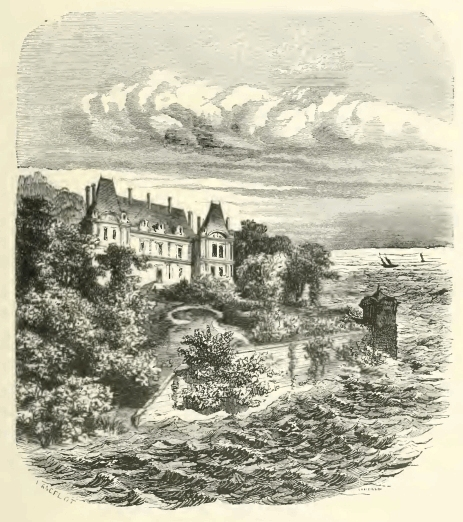
\includegraphics[width=\textwidth]{40188m.jpg}
\end{figure}

“Florentin here!” cried he, starting up; “is my mother ill?” And he
hastened to the door. Monte Cristo watched and saw him approach the
valet, who drew a small sealed parcel from his pocket, containing a
newspaper and a letter.

“From whom is this?” said he eagerly.

“From M. Beauchamp,” replied Florentin.

“Did he send you?”

“Yes, sir; he sent for me to his house, gave me money for my journey,
procured a horse, and made me promise not to stop till I had reached
you, I have come in fifteen hours.”

Albert opened the letter with fear, uttered a shriek on reading the
first line, and seized the paper. His sight was dimmed, his legs sank
under him, and he would have fallen had not Florentin supported him.

“Poor young man,” said Monte Cristo in a low voice; “it is then true
that the sin of the father shall fall on the children to the third and
fourth generation.”

Meanwhile Albert had revived, and, continuing to read, he threw back
his head, saying:

“Florentin, is your horse fit to return immediately?”

“It is a poor, lame post-horse.”

“In what state was the house when you left?”

“All was quiet, but on returning from M. Beauchamp’s, I found madame in
tears; she had sent for me to know when you would return. I told her my
orders from M. Beauchamp; she first extended her arms to prevent me,
but after a moment’s reflection, ‘Yes, go, Florentin,’ said she, ‘and
may he come quickly.’”

“Yes, my mother,” said Albert, “I will return, and woe to the infamous
wretch! But first of all I must get there.”

He went back to the room where he had left Monte Cristo. Five minutes
had sufficed to make a complete transformation in his appearance. His
voice had become rough and hoarse; his face was furrowed with wrinkles;
his eyes burned under the blue-veined lids, and he tottered like a
drunken man.

“Count,” said he, “I thank you for your hospitality, which I would
gladly have enjoyed longer; but I must return to Paris.”

“What has happened?”

“A great misfortune, more important to me than life. Don’t question me,
I beg of you, but lend me a horse.”

“My stables are at your command, viscount; but you will kill yourself
by riding on horseback. Take a post-chaise or a carriage.”

“No, it would delay me, and I need the fatigue you warn me of; it will
do me good.”

Albert reeled as if he had been shot, and fell on a chair near the
door. Monte Cristo did not see this second manifestation of physical
exhaustion; he was at the window, calling:

“Ali, a horse for M. de Morcerf—quick! he is in a hurry!”

\begin{figure}[ht]
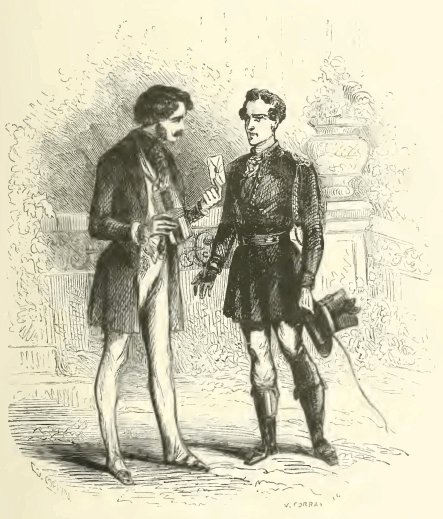
\includegraphics[width=\textwidth]{40190m.jpg}
\end{figure}

These words restored Albert; he darted from the room, followed by the
count.

“Thank you!” cried he, throwing himself on his horse.

“Return as soon as you can, Florentin. Must I use any password to
procure a horse?”

“Only dismount; another will be immediately saddled.”

Albert hesitated a moment. “You may think my departure strange and
foolish,” said the young man; “you do not know how a paragraph in a
newspaper may exasperate one. Read that,” said he, “when I am gone,
that you may not be witness of my anger.”

While the count picked up the paper he put spurs to his horse, which
leaped in astonishment at such an unusual stimulus, and shot away with
the rapidity of an arrow. The count watched him with a feeling of
compassion, and when he had completely disappeared, read as follows:

“The French officer in the service of Ali Pasha of Yanina alluded to
three weeks since in \textit{l’Impartial}, who not only surrendered the castle
of Yanina, but sold his benefactor to the Turks, styled himself truly
at that time Fernand, as our esteemed contemporary states; but he has
since added to his Christian name a title of nobility and a family
name. He now calls himself the Count of Morcerf, and ranks among the
peers.”

Thus the terrible secret, which Beauchamp had so generously destroyed,
appeared again like an armed phantom; and another paper, deriving its
information from some malicious source, had published two days after
Albert’s departure for Normandy the few lines which had rendered the
unfortunate young man almost crazy.
